\section{Representing Items}

A database was used to represent items, item sets, students, and student
responses.  A full diagrammatic representation of the database is shown in
Figure~\ref{fig:database}.

\begin{sidewaysfigure}[p!]
 \label{fig:database}
 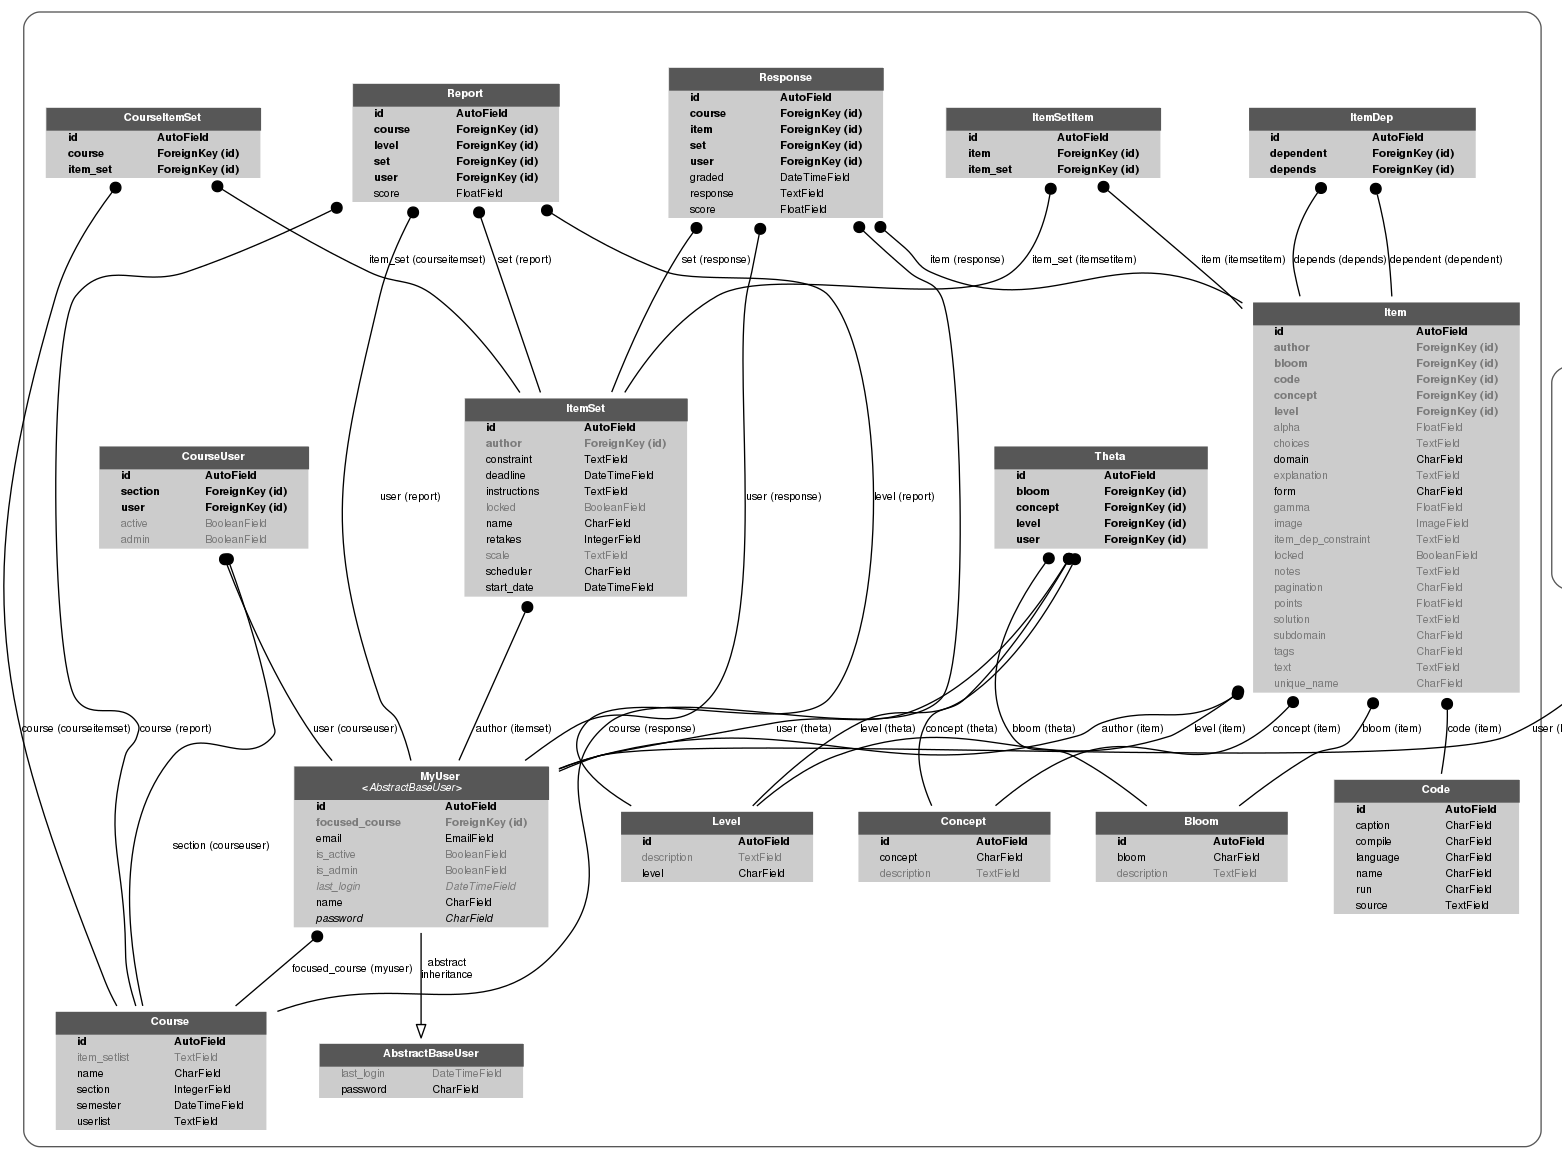
\includegraphics[width=9in]{fig/database.png} 
 \caption{The database layout.}

\end{sidewaysfigure}

The database contains items of the following nature:

\begin{itemize}

  \item \emph{Content}.  These include facts (which may be arranged into
  paragraphs, subsections, and sections), definitions, diagrams, and source
  codes.

  \item \emph{Assessment}.  These include questions, which may be true/false,
  multiple-choice, code writing, code simulation, short answer, and
  freewriting; also Likert scale items.

\end{itemize}

\subsection{Taxonomic Information}

Any output from this database to the student which is intended to solicit input
from the student has the following ordinal dimensions:

\begin{itemize}

  \item \emph{Difficulty}. Following the +/- grading system, difficulties range
  from -3 (very easy) to +3 (very hard), with 0 being medium. As alluded to
  earlier, difficulty determines the probability that a given student in the 
  class will answer the item correctly.

  \item \emph{Bloom level}.  The Bloom levels of cognitive functioning are
  Knowledge, Comprehension, Application, Analysis, Evaluation, and Synthesis.

  \item \emph{Concept}.  Concepts covered in computer science courses; for
  example in a programming course, these may include: Variables, Expressions,
  Control Structures, etc.

\end{itemize}

Any output to the student also has the following categorial dimensions:

\begin{itemize}

  \item \emph{Context}.  A problem may have a domain-specific context, e.g. it
  may be a problem relevant to biology, chemistry, physics, mathematics, etc.

  \item \emph{Type}.  The problem may be true/false, multiple-choice, short
  answer.

\end{itemize}

Each output may also have a dependency list, that is a list of IDs of, or a
rule describing, other output entries which the student should be exposed to
prior to that output.  For this system, Bloom level, subject domain, concept,
and difficulty are dimensions of a test question.  

It is important to note that the dimensions of the data are not necessarily
limited to the above; an exploratory factor analysis (EFA) could be used to
extend the dimensionality of the data semi-automatically.  This functionality
has not been implemented, but there exists a potential for it.


\subsection{Difficulty vs. Bloom Level}

With this, an alternative hypothesis is introduced: the Bloom cognitive
taxonomic level and the difficulty ($\beta$ value) are two separate properties
of items. Rather than being an indicator of difficulty, the Bloom level
indicates a cognitive dependency relationship to items at lower Bloom levels.

This is made clearer by the fact that Bloom levels are hierarchical: knowledge
is required for comprehension, comprehension is required for application, and
so forth.  At any level, there exists the potential to create items of a
range of difficulties. 

However, the application of Bloom's taxonomy to problems is specific to the
concept being analyzed, and moreover specific to the questions being asked.
The application of mathematical expressions (such as being able to evaluate or
reduce expressions) is different from the application of programmatic
expressions (being able to evaluate or reduce such expressions, bearing in mind
the language-specific rules).  The application of mathematical expressions
depends on the comprehension of mathematical expressions, however the
application problems may be easier once the dependencies are satisfied. 

Thus for every concept, and for every Bloom level, a student may possess a
different trait ability ($\theta$ value).  This explains why students would be
able to skip Bloom levels; in particular this would occur if a question of a
higher Bloom level (e.g. Evaluation) did not depend on the Bloom level
immediately preceding it (e.g. Analysis) but rather some lower level (e.g.
Application).  

A series of experiments have been conducted by the author toward the end of
supporting the hypothesis that Bloom levels represent dependency relationships
rather than difficulty levels \cite{castleberry2016effect}.  These experiments
consisted of demonstrating various ordering effects.  In the experiments,
questions of different Bloom levels (Knowledge through Evaluation) were asked
in forward and reverse order.  It was shown that forward-order schedules
resulted in statistically significantly greater performance than reverse-order
schedules \cite{castleberry2016effect}.   These experiments are detailed in
Sec~\ref{sec:experiments}.

